% 刚体

\pentry{矢量叉乘\upref{Cross}, 球坐标系\upref{Sph}, 质心\upref{CM}}

当我们要考虑一个物体的质量分布带来的力学效应时, 就不能再将其简化为一个质点. 许多情况下我们考虑的物体在某过程中形变较小可忽略不计, 这时我们就可以忽略它运动过程中的的任何形变, 从而大大简化问题. 我们把这种模型叫做\bb{刚体}. 在分析刚体时, 我们通常把刚体看做是质点系. 要这么做, 我们可以把刚体划分为无限多个体积无限小的微元, 再把每个微元近似为一个质量相同的质点即可. 

在没有任何约束的情况下, 每个质点有 3 个\bb{自由度}, 即用三个完全独立的变量才能完全确定位置, 所以 $N$ 个质点组成的质点系共有 $3N$ 个自由度. 然而完全确定一个刚体的位置只需要 6 个变量, 这是因为刚体模型通过假设“任意两个质点之间距离不变”, 给质点系的位置施加了 $3N - 6$ 个条件. 如何得出 6 个自由度呢? 我们可以假设第一个质点有 3 个自由度, 第二个质点由于要与第一个质点保持距离不变, 只有 2 个自由度, 而第三个质点要与前两个质点保持距离不变, 只有 1 个自由度. 有了前三个质点后(假设它们不共线), 剩下所有质点的位置都可以由与这三个质点的距离确定, 所以任何刚体都有 6 个自由度.

我们可以这么划分 6 个自由度: 令其中 3 个决定刚体质心的位置, 2 个决定过质心的某条轴的朝向(球坐标中的两个角度), 1 个决定刚体绕这条轴旋转的角度.

\subsection{刚体的绕轴转动}

若刚体绕固定轴转动, 那么刚体的位置只需一个变量即可完全确定(一个自由度), 我们令该变量为转角 $\theta$. $\theta$ 关于时间 $t$ 的导数就是刚体绕轴旋转的角速度 $\omega$. 我们不妨再定义角速度 $\omega$ 关于时间的导数(即 $\theta$ 关于时间的二阶导数)为\bb{角加速度}, 记为 $\alpha$.

我们可以把刚体的绕轴转动类比质点的直线运动, 把 $\theta$, $\omega$ 和 $\alpha$ 分别类比为直线运动中的位置 $x$, 速度 $v$ 和 加速度 $a$, 因为后三个变量之间的数学关系是完全相同的. 于是我们可以立即得到匀变速转动(即 $\alpha$ 为常数)的一些公式, 如
\begin{gather}
\theta = \theta_0 + \omega t + \frac12 \alpha t^2\\
\omega_1^2 - \omega_0^2 = 2\alpha \theta
\end{gather}

在以上三个标量的基础上, 我们可以定义它们的矢量形式 $\vec \theta$, $\vec \omega$ 和 $\vec \alpha$, 令它们的方向为转轴的方向, 用右手定则\upref{RHRul} 来判断.

\begin{figure}[ht]
\centering
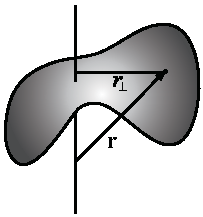
\includegraphics[width=4cm]{./figures/RigBd1.pdf}
\caption{刚体绕轴旋转时任意一点的线速度} \label{RigBd_fig1}
\end{figure}

我们再来考虑刚体旋转时其中任意一点的瞬时速度(如\autoref{RigBd_fig1}). 显然刚体绕轴旋转时, 刚体中不在轴上的点都做圆周运动, 速度大小为 $\omega \cross r_{\bot}$. 其中 $r_{\bot}$ 是该点到转轴的垂直距离. 如果令 $\vec r$ 为转轴上任意一点指向刚体中某点的矢量, 根据矢量叉乘\upref{Cross}的几何定义, 该点的瞬时线速度可以表示为
\begin{equation}
\vec v = \vec r \cross \vec \omega
\end{equation}
